\documentclass[journal, a4paper]{IEEEtran}
%\usepackage{cite} %Waiting for MikTeX to feel better
\usepackage{amsmath}
\usepackage{amssymb}
\usepackage{graphicx}
%\usepackage{hyperref}
\usepackage[version=3]{mhchem}
\usepackage[numbers, sort&compress]{natbib}
\usepackage{units}
\usepackage{upgreek}
%Wave 2
\usepackage[caption=false]{subfig}

\renewcommand{\d}{\ensuremath{\mathrm{d}}}
\let\originalleft\left
\let\originalright\right
\renewcommand{\left}{\mathopen{}\mathclose\bgroup\originalleft}
\renewcommand{\right}{\aftergroup\egroup\originalright}


\pdfsuppresswarningpagegroup=1 %pagegroup warning

\title{Optical Characterisation of a Strained-Silicon Cold-Electron Bolometer at 160 GHz}
\author{\IEEEauthorblockN{%
T. L. R. Brien\IEEEauthorrefmark{1}\thanks{E-mail: tom.brien@astro.cf.ac.uk}, %
P. A. R. Ade\IEEEauthorrefmark{1}, %
P. S. Barry\IEEEauthorrefmark{1}, %
C. J. Dunscombe\IEEEauthorrefmark{1}, %
D. R. Leadley\IEEEauthorrefmark{2}, %
D. V. Morozov\IEEEauthorrefmark{1},\\%
M. Myronov\IEEEauthorrefmark{2}, %
E. H. C. Parker\IEEEauthorrefmark{2}, %
M. J. Prest\IEEEauthorrefmark{2}\IEEEauthorrefmark{3}, %
M. Prunnila\IEEEauthorrefmark{4}, %
R. V. Sudiwala\IEEEauthorrefmark{1},\\%
T. E. Whall\IEEEauthorrefmark{2} and %
P. D. Mauskopf\IEEEauthorrefmark{1}\IEEEauthorrefmark{5}}
\\%
\IEEEauthorblockA{\IEEEauthorrefmark{1}School of Physics and Astronomy,%
Cardiff University, The Parade,%
Cardiff, CF24 3AA, UK}\\%
\IEEEauthorblockA{\IEEEauthorrefmark{2}Department of Physics,%
 University of Warwick, Coventry,%
 CV4 7AL, UK}\\%
\IEEEauthorblockA{\IEEEauthorrefmark{3}School of Engineering,%
Cardiff University, The Parade,%
Cardiff, CF24 3AA, UK}\\%
\IEEEauthorblockA{\IEEEauthorrefmark{4}VTT Technical Research Centre of Finland, P.O. Box 1000, FI-02044 VTT Espoo, Finland}\\%
\IEEEauthorblockA{\IEEEauthorrefmark{5}Department of Physics and School of Earth \& Space Exploration,%
 Arizona State University,\\ 650 E. Tyler Mall, Tempe, AZ 85287, USA}
}
\IEEEpubid{978-1-4673-7434-7/15/\$31.00~\copyright2015 IEEE}
\date{\today}
\begin{document}
\maketitle
\begin{abstract}
\boldmath
We present a study of a cold-electron bolometer operating at $350~\mathrm{mK}$  with a twin-slot antenna coupling radiation at $160~\mathrm{GHz}$. The detector's absorbing element consists of degenerately-doped strained silicon and has Schottky contacts to superconducting aluminium leads. These contacts allow for direct electron cooling of the absorber to below the phonon temperature, enabling the cold-electron bolometer to achieve much faster time constants ($\tau < 1~\mathrm{\upmu s}$) compared to conventional bolometric detectors while not sacrificing sensitivity. We measure both the dark and optically-loaded noise of the detector via a novel method of cross-correlating the outputs of two amplifiers in order to measure noise below the amplifier noise level. From this we measure the photon-noise limited noise-equivalent power of the detector to be $6.6 \times 10^{-17}~\mathrm{W\,Hz^{\nicefrac{-1}{2}}}$ when observing a 77-Kelvin source.
\end{abstract}
\section{Introduction}
At low temperatures the thermal coupling between the electron and phonon systems in a material becomes weak. The idea of combining this with a sensitive normal metal-insulator-superconductor (NIS) junction thermometer to make a sensitive hot-electron bolometer was first proposed by Nahum, Richards and Mears \cite{Nahum1993}. Furthermore, combining weak electron-phonon coupling in a material with tunnelling contacts has been shown to enable cooling of the electrons in the material to below the lattice temperature \cite{Nahum1994}. By combining these two complimentary technologies one can create a so-called cold-electron bolometer, where the electrons in the absorbing element are directly cooled by a set of NIS junctions. This allows the detector to exhibit high sensitivities (due to the excellent thermal isolation between electrons and phonons) without sacrificing detector speed. Such a device was first described by Kuzmin, Devyatov and Golubev \cite{Kuzmin1998}. Savin showed that if one replaces the cooled metallic island with a highly-doped semiconductor, the achieved minimum electron temperature is lower due to the weaker electron-phonon coupling in the semiconductor compared to the metal \cite{Savin2001}. Such a configuration has the added advantage that the NIS junctions to the island can be replaced by naturally forming Schottky barriers, thus simplifying the fabrication. Development of cold-electron bolometers has been accelerating in recent years to the stage where optical measurements using both metallic and semiconducting absorbers have now been reported \cite{Tarasov2011,Otto2013,Brien2014}. A novel development in this field is the use of a degenerately-doped strained-silicon
absorber, which has been shown to improve electron cooling compared to unstrained materials \cite{Prest2011}.
\par 
In this work we present a detailed study of a strained-silicon cold-electron bolometer by measuring the noise-equivalent power (NEP) both in the absence of optical power, and when observing 77- and 300-Kelvin sources. These measurements have been performed using a novel system of cross-correlating the output of two matched JFET amplifiers to enable measurements below the noise limit of a single amplifier. This work presents a more detailed study of both the responsivity and the sensitivity across the whole operational range bias range of the device, compared to Ref.~\citenum{Brien2014}.
\section{Theory}
A cold-electron bolometer selectively removes the most energetic (hottest) electrons from the absorber. For a silicon-based cold-electron bolometer these electrons tunnel out of the absorber through Schottky barriers to the superconducting contacts. A typical energy diagram for a detector biased such that there is a voltage $V$ across the device is shown in Fig.~\ref{fig:CEBenergy}.  In the absence of any bias, the Fermi energy is the same in the absorber and the superconducting contacts and thus carriers cannot tunnel between the two since this corresponds to the gap states in the superconductor. However, in the presence of an external bias, applied across the structure, the Fermi level in the superconductor can be moved relative to that of the absorber, allowing tunnelling from the absorber to the vacant states above the superconductor's energy gap. Intelligent selection of the bias level allows for only the most energetic (the hottest) electrons to tunnel from the
\newpage \noindent
central island, these are replaced by lower-energy electrons from the sub-gap states in the superconducting contact, thus reducing the overall energy (cooling) of the absorber. 
\begin{figure}[tb]
\centering 
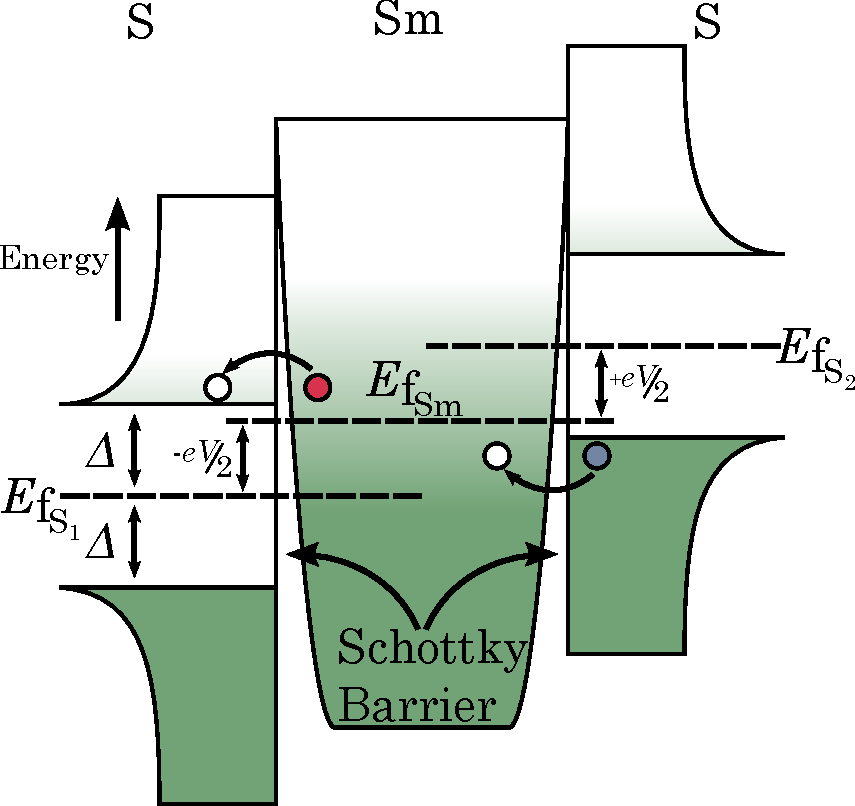
\includegraphics[width = 0.65\columnwidth]{CEB_energyLevels_bias}
\caption{Energy bands for a biased superconductor-semiconductor-superconductor structure (SSmS). In order for electrons to tunnel out of the central semiconducting absorber and into the lower-energy superconductor (left), we require that  $eV/2 > \varDelta - k_{\mathrm{B}}T_{\mathrm{e}}$ , where $V$  is the voltage across the two junctions due to the bias, $T_{\mathrm{e}}$ is the electron temperature and $\varDelta $ is half the superconducting gap.}
\label{fig:CEBenergy}
\end{figure}
 \par 	
In the structure illustrated in Fig.~\ref{fig:CEBenergy}, the current, $I$, flowing through each of the junctions is given by:
\begin{align}
I = \frac{1}{eR_{\mathrm{N}}}\int^{\infty}_{\varDelta} 
	&\frac{E}{\sqrt{E^{2}-\varDelta^{2}}} \times 
	\left[f\left(\!E-eV/2,T_{\mathrm{e}}\right)\right. \nonumber \\
	&\left. - f\left(\!E+eV/2,T_{\mathrm{e}}\right)\right]\,\mathrm{d}E\,,
	\label{eqn:IV}
\end{align}
where $R_{\mathrm{N}}$ is the normal-state resistance, due to tunnelling, of an individual tunnelling barrier, $\varDelta$ is half the superconducting bandgap, $V$ is the voltage across both junctions, and $f\!\left(E,T\right)$ is the Fermi distribution of electrons at temperature $T_{\mathrm{e}}$ and this tunnelling current either increases or decreases the average energy of the electrons in the absorber. This change in energy can be expressed as a tunnelling power, $P$, given by:
\begin{align}
P = IV &+\frac{2}{e^{2}R_{\mathrm{N}}}\int^{\infty}_{\varDelta}\frac{E^{2}}
	{\sqrt{E^{2}-\varDelta^{2}}} \times \left[2\,f\!\left(E,T_{\mathrm{s}}\right)
	\right.\nonumber \\
	&\left. - f\!\left(E-eV/2,T_{\mathrm{e}}\right)
	- f\!\left(E+eV/2,T_{\mathrm{e}}\right)\right]\,\mathrm{d}E\,,
	\label{eqn:Ptun}
\end{align}
where $T_{\mathrm{s}}$ is the temperature of the normal-state electrons in the superconductor. A negative value of $P$ represents a net reduction in the energy of the electrons in the absorber and thus corresponds to electron cooling.
\par 
It is this tunnelling power that cools the absorber and, when operating as a detector, may be used to remove the incident optical power. The tunnelling current (Eqn~\ref{eqn:IV}) is exponentially dependant upon the temperature of the electrons, $T_{\mathrm{e}}$, and thus acts as a highly-sensitive thermometer.
\par 
The weak thermal link between the electrons and phonons causes a power flow between the two systems which is given by:
\begin{align}
P_{\mathrm{e\mbox{-}ph}} = \varSigma\varOmega
	\left(T_{\mathrm{e}}^{\beta} - T_{\mathrm{ph}}^{\beta}\right)\,
\end{align}
where $\varSigma$ is a material constant, $\varOmega$ is the volume of the bolometer's absorber, and $T_{\mathrm{e}}$ and $T_{\mathrm{ph}}$ are the temperatures of the electrons and phonons respectively. The value of $\varSigma$ for the strained material used here is $2 \times 10^{7}~\mathrm{W\,K^{-6}\,m^{-3}}$ and that the power $\beta$ is equal to $6$ \cite{Muhonen2011,Prest2011}. The thermal conduction from the phonon system to the electrons can thus be defined as:
\begin{align}
G_{\mathrm{e\mbox{-}ph}} = \frac{\d P_{\mathrm{e\mbox{-}ph}}}{\d T_{\mathrm{e}}}
	= \beta\varSigma\varOmega T_{\mathrm{e}}^{\beta-1}\,.
\end{align}
\par 
The noise performance, in the absence of any optical power, is limited by fluctuations in both this heat flow between electrons and phonons and the rate at which electrons tunnel into and out of the semiconducting absorber. A full treatment of this is given by Golubev and Kuzmin \cite{Golubev2001} and, with the addition of amplifier voltage noise, $\left<\delta V^{2}\right>_{\mathrm{amp}}$, the dark noise-equivalent power is:
\begin{align}
\textit{NEP}_{\mathrm{CEB}}^{2} 
	= &\frac{\left<\delta V^{2}\right>_{\mathrm{amp}}}{S_{\mathrm{V}}^{2}}
	+ 2\beta k_{\mathrm{B}}\varSigma\varOmega\left(T_{\mathrm{e}}^{\beta+1}
		+T_{\mathrm{ph}}^{\beta+1}\right)\nonumber\\
	&+\left<\delta P^{2}\right>
	+\frac{\left<\delta I^{2}\right>}
		{\left(\frac{\partial I}{\partial V}S_{\mathrm{V}}\right)^{2}}
	-2\frac{\left<\delta P \delta I\right>}
		{\frac{\partial I}{\partial V}S_{\mathrm{V}}}\,, \label{eqn:NEP}
\end{align}
where $S_{\mathrm{V}}$ is the voltage responsivity of the detector, $\left<\delta I\right>$ and $\left<\delta P\right>$ are the fluctuations in the tunnelling current and noise respectively, and $2\left<\delta P \delta I\right>$ is the correlator of these two quantities. Eqn~\ref{eqn:NEP} directly illustrates the advantage of strained silicon since the value of $\varSigma$ is a factor of $25$ lower compared to unstrained silicon \cite{Prest2011}. In any operational scenario additional noise is also introduced by the absorption of photons in the absorber. This is given by the well-known expression:
\begin{align}
\textit{NEP}_{\mathrm{photon}}^{2} = 2h\nu P_{\mathrm{opt}} 
	+ \frac{P_{\mathrm{opt}}^{2}}{\delta\nu}\,,
\label{eqn:photonNoise}
\end{align}
where $P_{\mathrm{opt}}$ is the optical power, $h$ is Planck's constant, and $\nu$ and $\delta\nu$ and the frequency and bandwidth of the incident light.
\par 
Golubev and Kuzmin \cite{Golubev2001} also give an equation for the voltage responsivity, which when adapted to the DC limit, is given by:
\begin{align}
S_{\mathrm{V}} = 
	\frac{\frac{-\frac{\partial I}{\partial T_{\mathrm{e}}}}
		{\frac{\partial I}{\partial V}}}
	{\beta\varSigma\varOmega T_{\mathrm{e}}^{\beta-1}
		+\frac{\frac{\partial I}{\partial T_{\mathrm{e}}}}
		{\frac{\partial I}{\partial V}}\frac{\partial P}{\partial V}
	-\frac{\partial P}{\partial T_{\mathrm{e}}}}\,. \label{eqn:responsivity}
\end{align}
%
\section{Device Structure}
The device is fabricated from a wafer consisting of a $30~\mathrm{nm}$ layer of  highly-doped ($N_{\mathrm{D}} = 4 \times 10^{19}~\mathrm{cm^{-3}}$) silicon which is strained via a $2.5~\mathrm{\upmu m}$ layer of \ce{Si_{0.8}Ge_{0.2}}. Detector designs are patterned via photo lithography and wet etching processes. The aluminium, which forms the contacts to the strained-silicon absorber as well as the antenna, is deposited via sputtering and then patterned in a similar manner to the silicon. After fabrication the area of the absorber is $32 \times 14~\mathrm{\upmu m}$. It should be noted that this is comparatively large proof-of-concept device. A cross section of the final device structure, along with an optical photograph, is shown in Fig.~\ref{fig:device}.
\begin{figure}[ht]
\begin{center}
\subfloat[]{
	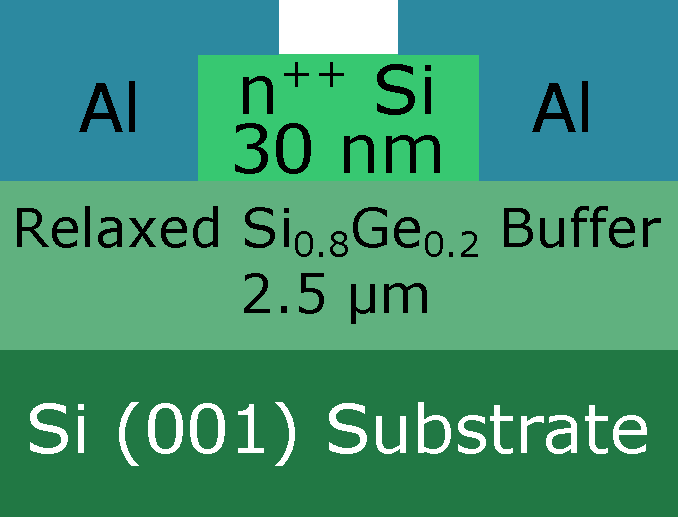
\includegraphics[width=0.3\columnwidth]{crossSection}
	\label{fig:crossSection}
}
\subfloat[]{
	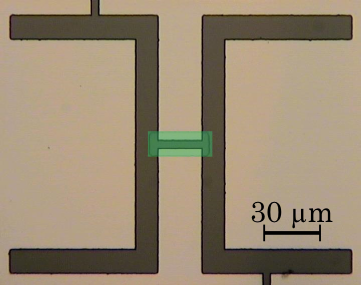
\includegraphics[width=0.3\columnwidth]{devicePhoto}
	\label{fig:devicePhoto}
}
\caption{(a) Cross section of fabricated detector structure. (b) Optical photograph of detector structure with absorber highlighted for clarity.}
\label{fig:device}
\end{center}
\end{figure}
%
\section{Experimental Setup}
Measurements of the strained-silicon cold-electron bolometer have been taken in both a dark environment and in the presence of optical illumination. All measurements were performed in a liquid-helium cryostat with the device further cooled by a two-stage helium sorption refrigerator such that the base operating temperature of the detector was $350~\mathrm{mK}$. For optical measurements the optical bandwidth has been defined by a set of filters fabricated in house at Cardiff. These filters act to reduce the optical radiation incident on the detector to a low-pass edge of $300~\mathrm{GHz}$. In addition to the detector's twin-slot antenna, radiation was further focused onto the detector chip via a hyper-extended hemispherical silicon lens and a pair of back-to-back horns. A schematic of the optical testing configuration is shown in Fig.~\ref{fig:setup}.
\begin{figure}[htb]
\begin{center}
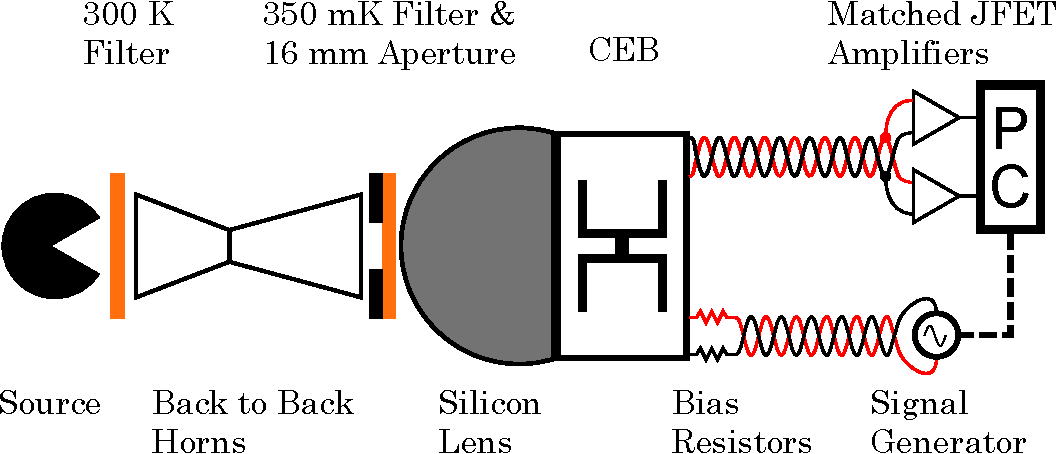
\includegraphics[width=0.8\columnwidth]{experimental_setup}
\caption{Experimental setup for optical measurements. Light is coupled to the detector via a set of back-to-back horns and a silicon leans. A set of optical filters limit the incident radiation to an upper frequency of $300~\mathrm{GHz}$. Bias is provided to the device via a simple configuration of a programmable voltage source and a set of cold biasing resistors. The output of the detector is split and fed to a pair of matched JFET amplifiers whose outputs are fed to a computer and cross correlated.}
\label{fig:setup}
\end{center}
\end{figure}
\par 
In order to measure the detector noise, which for this device was of the order of $< 1~\mathrm{nV\,Hz^{\nicefrac{-1}{2}}}$ we have utilised a novel readout system whereby the output of the detector is split and fed in parallel to two matched JFET amplifiers, the outputs of these are then fed to a computer where they a cross-correlated. This cross-correlation dramatically reduces the amplifier noise, since the noise of the two amplifiers is uncorrelated, and leaves the device noise (correlated at both amplifiers) clearly examinable. The overall effect of this technique is to reduce the amplifier noise from the single-amplifier limit of $1~\mathrm{nV\,Hz^{\nicefrac{-1}{2}}}$ for the amplifiers used here to a level of $300~\mathrm{pV\,Hz^{\nicefrac{1}{2}}}$, this remaining level is due to stray capacitances weakly coupling the amplifier noise back into the detector producing a low level of correlated noise between the two amplifiers.% The reduction in amplifier noise with increased averaging is shown in Fig.~\ref{fig:ampNoise}.
%\begin{figure}[htb]
%\begin{center}
%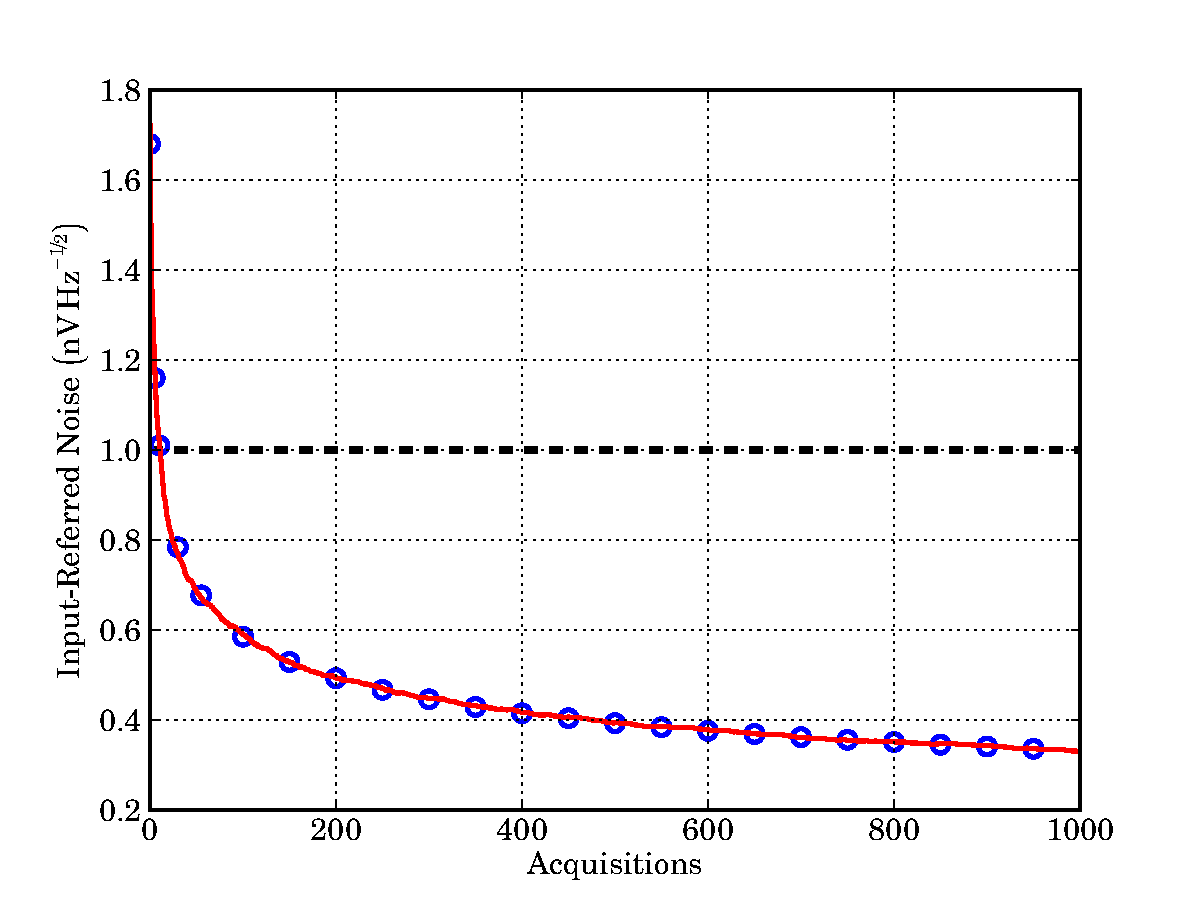
\includegraphics[width=0.9\columnwidth]{crossColNoiseSimData}
%\caption{Improvement in amplifier noise with cross-correlation for increased %number of acquisitions. Line - data, cirles - model.}
%\label{fig:ampNoise}
%\end{center}
%\end{figure}
%
\section{Results \& Discussion}
Measurements of the $I$-$V$ characteristics of the detector have been carried out both dark and optically loaded. These show that at voltage levels lower than $\pm 2\varDelta$ ($\approx 360~\mathrm{\upmu eV}$) the detector exhibits high resistance. As the voltage is further increased the situation illustrated in Fig.\ref{fig:CEBenergy} arises and the tunnelling rate of electrons dramatically increases. This results in a  lower resistance. $I$-$V$ curves have been recorded dark for numerous bath temperatures and in the presence of optical loading from 77-Kelvin and room-temperature sources and a summary of these results are presented in Fig.~\ref{fig:IV}. It can be seen that the effect of increasing the optical power is similar to that of increasing the bath temperature (i.e. the $I$-$V$ curve shifts towards the linear), indeed the $I$-$V$ curve for the 77-Kelvin illumination ($T_{\mathrm{bath}} = 350~\mathrm{mK}$) is comparable to the dark $I$-$V$ curve measured at $550~\mathrm{mK}$.
\begin{figure}[htb]
\begin{center}
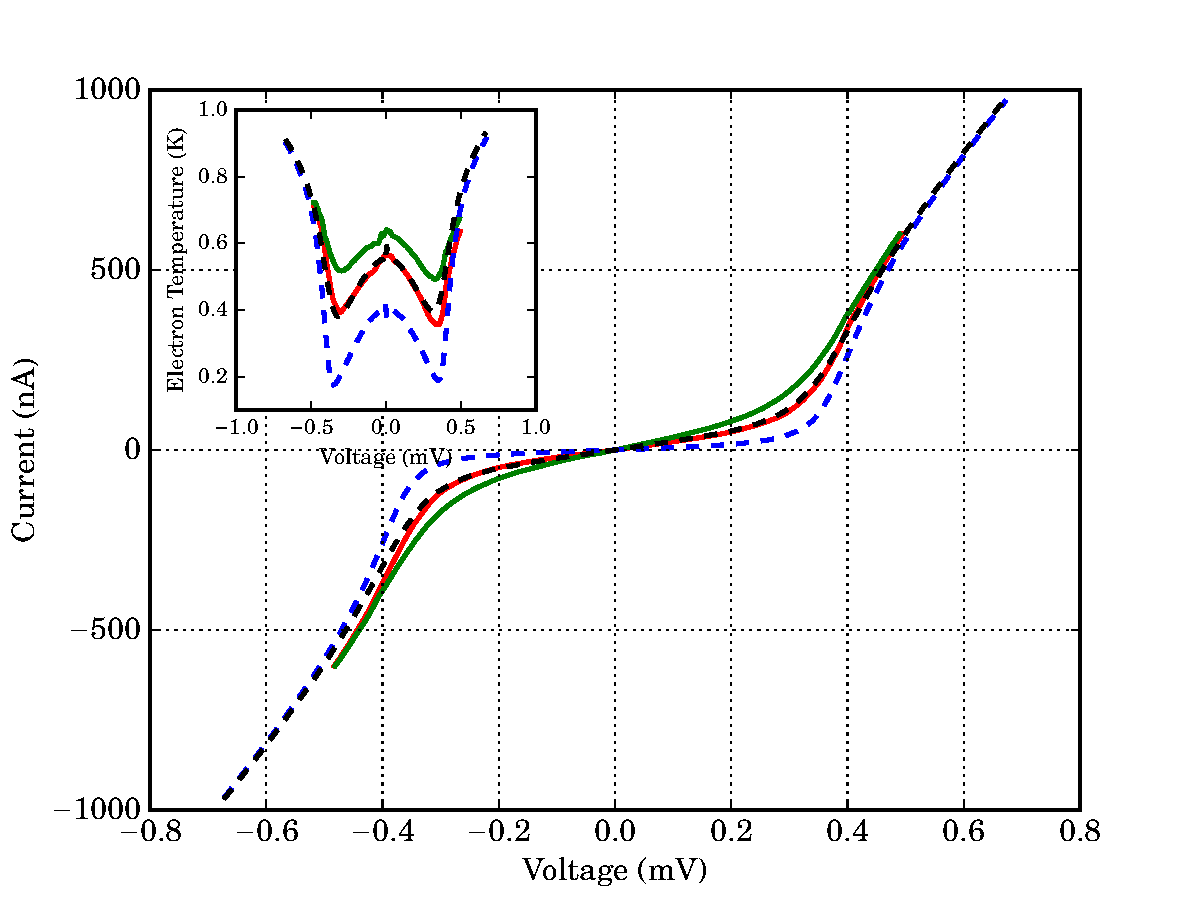
\includegraphics[width=0.9\columnwidth]{IVs}
\caption{$I$-$V$ characteristics. Dashed lines: dark data, blue - $T_{\mathrm{bath}} = 350~\mathrm{mK}$, black - $550~\mathrm{mK}$. Solid lines: optically loaded data $T_{\mathrm{bath}} = 350~\mathrm{mK}$, red - 77-Kelvin source, green - room-temperature source. Inset: electron temperature, colours as in main figure.}
\label{fig:IV}
\end{center}
\end{figure}
\par 
From fitting the data shown in Fig.~\ref{fig:IV} to Eqn~\ref{eqn:IV} it is possible to calculate the electron temperature at each data point, this is shown in the inset of Fig.~\ref{fig:IV} and by taking the difference between the bath temperature and the electron temperature at zero bias it is possible to calculate the power absorbed within the detector. Doing so we find the absorbed power from the 77-Kelvin source to be $9.2~\mathrm{pW}$ and $20.0~\mathrm{pW}$ for the room-temperature illumination.
\par 
From these results and Eqn~\ref{eqn:responsivity} it was possible to calculate the responsivity for the detector under the two optical loadings. This is shown in Fig.~\ref{fig:responsivity}. The peak responsivity when observing the room-temperature source was $4.7 \times 10^{6}~\mathrm{V\,W^{-1}}$, whereas for the 77-Kelvin source it was $1.5 \times 10^{7}~\mathrm{V\,W^{-1}}$. This reduction for the higher-power load is the result of the tunnelling power being unable to fully remove all the incident power at the higher level.
\begin{figure}[tb]
\begin{center}
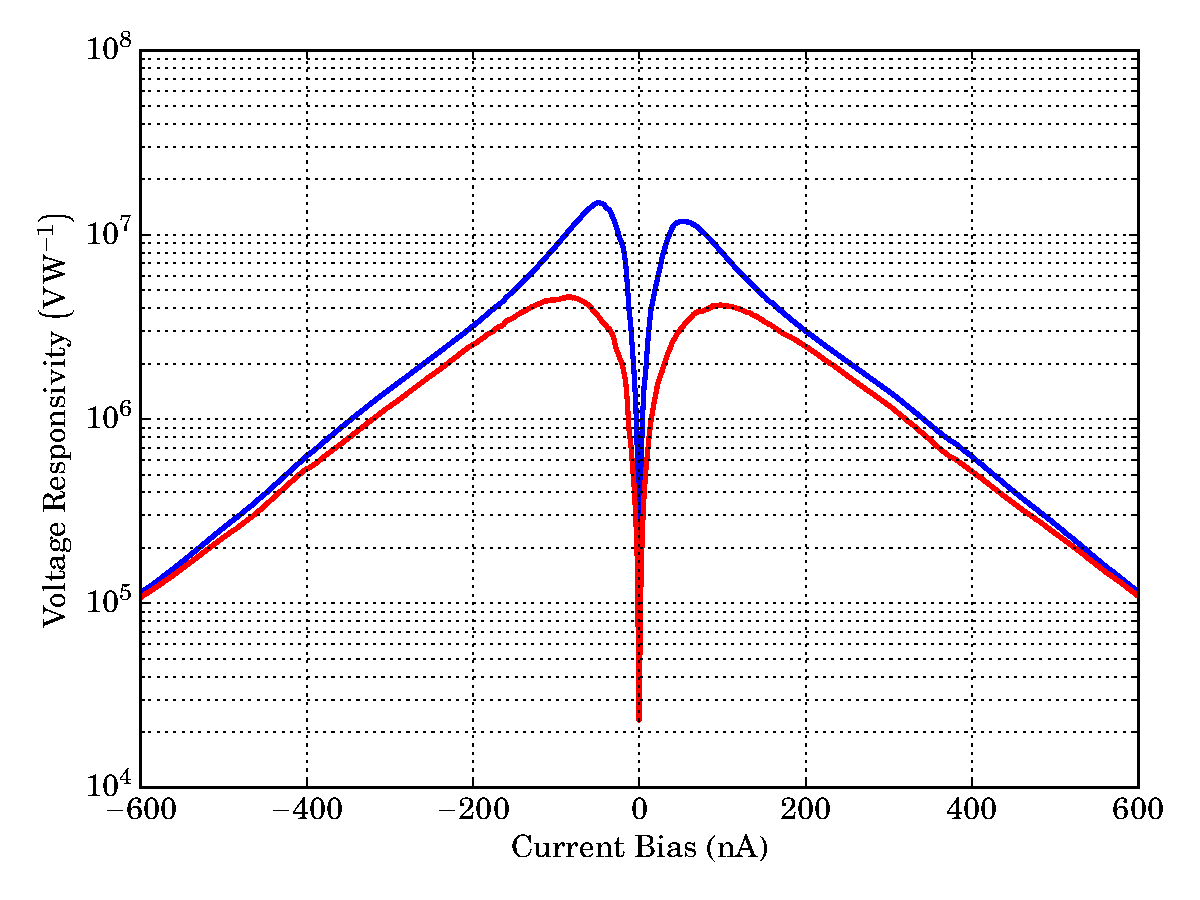
\includegraphics[width=0.9\columnwidth]{responsivity}
\caption{Detector responsivity for the device when illuminated by a 77-Kelvin (blue) and room-temperature (red) source. The slight asymmetry is most likely the result of a minor misalignment during fabrication.}
\label{fig:responsivity}
\end{center}
\end{figure}
\par 
Finally, by using the noise model presented in Eqn~\ref{eqn:NEP} we have produced a model for the noise-equivalent power of this detector as a function of operating voltage. This has been compared to data taken by measuring the device noise at various bias points and using the results presented in Fig.~\ref{fig:responsivity} to calculate the noise-equivalent power. This is shown for the 77-Kelvin illumination in Fig.~\ref{fig:NEP}. Uncertainties have been calculated for the data points from combining the uncertainty in the responsivity with the uncertainty arising from the noise measurement.
\begin{figure}[tb]
\begin{center}
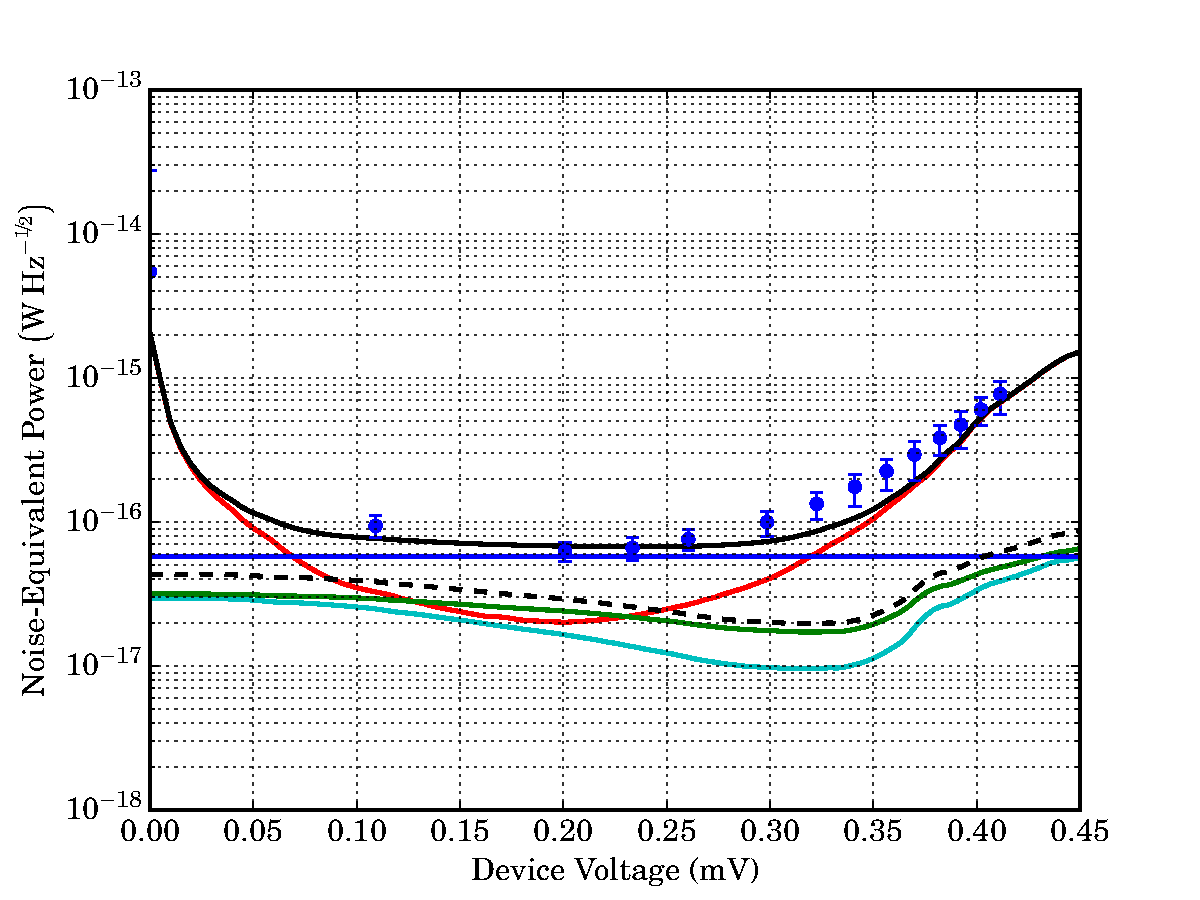
\includegraphics[width=0.9\columnwidth]{noiseModel}
\caption{Noise-equivalent power of a strained-silicon cold-electron bolometer. Lines: model, cyan - electron-phonon noise, green - tunnelling noise, red - amplifier noise, blue - photon noise, dashed black - total device noise, solid black - total noise. Circles: measured data. Note that the device is photon noise limited for operating voltages between $0.07$ and $0.32~\mathrm{mV}$.}
\label{fig:NEP}
\end{center}
\end{figure}
\par 
Fig.~\ref{fig:NEP} shows excellent agreement between our model and our data overall and shows that between voltages of $0.07$ and $0.32~\mathrm{mV}$ the detector is photon noise dominated with a minimum noise-equivalent power of $6.6 \times 10^{-17}~\mathrm{W\,Hz^{\nicefrac{-1}{2}}}$. Our model shows that in the absence of noise from the amplifier or from photons, the dark noise-equivalent power (dashed line in Fig.~\ref{fig:NEP}) is $2 \times 10^{-17}~\mathrm{W\,Hz^{\nicefrac{-1}{2}}}$. Repeating the same analysis for the room-temperature illumination yields similar results. In this case the minimum noise-equivalent power was $1.3 \times 10^{-16}~\mathrm{W\,Hz^{\nicefrac{-1}{2}}}$. This is to be expected from the lower responsivity shown in Fig.~\ref{fig:responsivity} for this illumination.
By measuring the roll off of the noise in the photon noise limited region we ascertain that the speed of the device is $<1~\mathrm{\upmu s}$, the bandwidth limit of our amplifier.
%
\newpage
\section{Conclusions}
We have measured the optical response of a strained-silicon cold-electron bolometer to two optical sources. We have found that the noise-equivalent power of this detector has a minimum value of $6.6 \times 10^{-17}~\mathrm{W\,Hz^{\nicefrac{-1}{2}}}$ when observing a 77-Kelvin optical source and is limited by photon noise; in the absence of photon and amplifier noise the dark noise-equivalent power is $2 \times 10^{-17}~\mathrm{W\,Hz^{\nicefrac{-1}{2}}}$. This has been performed by using a novel method of cross-correlating the output of two amplifiers to measure below the noise level of a single amplifier.
%
\section*{Acknowledgements}
This work has been financially supported by the STFC through Grant ST/K000926/1, the EPSRC through grant numbers EP/F040784/1 and EP/J001074/1, and the Academy of Finland through Grant 252598. 
%
\bibliographystyle{IEEEtran}
\bibliography{bib}

\end{document}
